\documentclass[tikz,border=4pt]{standalone}
\usepackage{amsmath,amssymb}
\usepackage{pgfplots}\pgfplotsset{compat=1.18}\usepgfplotslibrary{polar}
\usetikzlibrary{arrows.meta,positioning,automata,shapes,shapes.misc,calc,decorations.pathmorphing,decorations.markings,angles,quotes,patterns,mindmap,matrix,knots,hobby,trees}
\tikzset{->-/.style={decoration={markings, mark=at position 0.5 with {\arrow{Stealth}}}, postaction={decorate}}}
\begin{document}
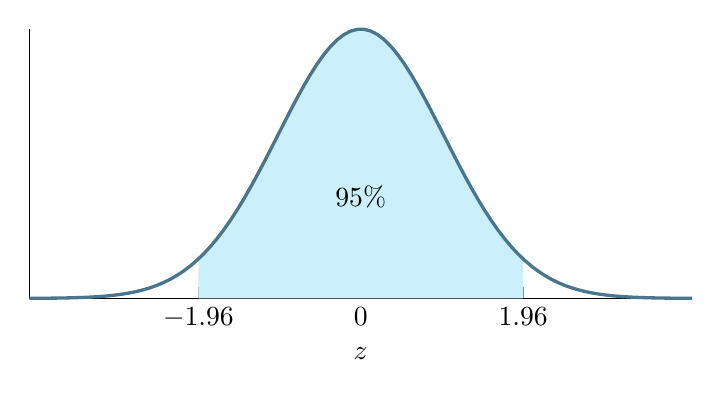
\begin{tikzpicture}
\begin{axis}[no markers, domain=-4:4, samples=100, axis lines*=left, xlabel=$z$, height=5cm, width=10cm, xtick={-1.96,0,1.96}, xticklabels={$-1.96$,$0$,$1.96$}, ytick=\empty, enlargelimits=false, clip=false]
\addplot[fill=cyan!20, draw=none, domain=-1.96:1.96] {exp(-x^2/2)/sqrt(2*pi)} \closedcycle;
\addplot[very thick, cyan!50!black] {exp(-x^2/2)/sqrt(2*pi)};
\node at (axis cs:0,0.15) {$95\%$};
\end{axis}
\end{tikzpicture}
\end{document}
